%===============================================================================
\chapter{Statistical Field Theory: The O(N) Model}
\label{ch:on_model}
%===============================================================================

The O(N) model is the canonical example for perturbative RG in statistical field theory, and this chapter applies the six-step recipe of Chapter~\ref{ch:recipe} in detail. The model describes systems with an N-component order parameter and exhibits a rich phase structure including continuous phase transitions. By working through the recipe systematically, we will see how the abstract framework of Part I produces concrete predictions for critical exponents that have been verified experimentally.

The scale hierarchy (Step 1) ranges from the UV cutoff $\Lambda$ (the lattice scale) to the IR correlation length $\xi$. Coarse-graining (Step 2) proceeds by integrating out high-momentum modes in thin shells, the Wilsonian approach. Theory space (Step 3) is parametrized by the mass-squared $r$ and quartic coupling $u$. The beta functions (Step 4) are computed perturbatively using the $\epsilon$-expansion. Fixed-point analysis (Step 5) reveals the Gaussian and Wilson-Fisher fixed points, with the latter controlling critical behavior in $d < 4$.

\marginnote{The O(N) model encompasses many physical systems: $N=1$ is Ising, $N=2$ is XY (superfluids), $N=3$ is Heisenberg (magnets), $N=4$ is relevant to electroweak theory.}

%-------------------------------------------------------------------------------
\section{The O(N) Symmetric Field Theory}
\label{sec:on_lagrangian}
%-------------------------------------------------------------------------------

The Euclidean action for the O(N) model in $d$ dimensions is
\begin{equation}
S[\phi] = \int d^d x \left[ \frac{1}{2}(\partial_\mu \phi^a)(\partial^\mu \phi^a) + \frac{r_0}{2}\phi^a \phi^a + \frac{u_0}{4!}(\phi^a \phi^a)^2 \right]
\label{eq:on_action}
\end{equation}
where $\phi^a$ ($a = 1, \ldots, N$) is an N-component real scalar field, $r_0$ is the bare mass squared, and $u_0$ is the bare quartic coupling. Repeated indices are summed.

\subsection{Scale Identification}

Following Step 1 of the recipe, we identify the scales. The momentum cutoff $\Lambda$ provides the UV scale where the continuum description breaks down, typically corresponding to the inverse lattice spacing in a microscopic model. The correlation length $\xi$ provides the IR scale characterizing the decay of correlations, which diverges at the critical point.

The scale parameter $s = \ln(\Lambda/\mu)$ measures the logarithm of the ratio between the cutoff and the renormalization scale $\mu$. As we integrate out modes and reduce the effective cutoff, $s$ increases. The dimensionless couplings $r = r_0/\Lambda^2$ and $u = u_0 \Lambda^{d-4}$ are the natural variables for the RG, with the powers of $\Lambda$ chosen to make them dimensionless in $d$ dimensions.

%-------------------------------------------------------------------------------
\section{Canonical Scaling Dimensions}
\label{sec:on_canonical}
%-------------------------------------------------------------------------------

From the action~\eqref{eq:on_action}, we read off the canonical (engineering) dimensions using the principle of Chapter~\ref{ch:flows}.

For the action to be dimensionless:
\begin{equation}
[\phi] = \frac{d-2}{2}, \quad [r_0] = 2, \quad [u_0] = 4 - d.
\end{equation}

\marginnote{The canonical dimension of $u_0$ determines whether the $\phi^4$ interaction is relevant, irrelevant, or marginal at the Gaussian fixed point.}

The critical dimension $d_c = 4$ is where $u_0$ becomes dimensionless. For $d < 4$, the coupling is relevant at the Gaussian fixed point, driving the system to a nontrivial interacting fixed point.

%-------------------------------------------------------------------------------
\section{The Wilson-Fisher Fixed Point}
\label{sec:wilson_fisher}
%-------------------------------------------------------------------------------

We now derive the famous Wilson-Fisher fixed point using the $\varepsilon$-expansion, where $\varepsilon = 4 - d$.

\subsection{One-Loop Beta Functions}

Using standard perturbative techniques involving dimensional regularization and the minimal subtraction scheme, the beta functions to one loop are:
\begin{align}
\beta_r &\equiv \mu \frac{\partial r}{\partial \mu} = -2r + \frac{(N+2)u}{6(4\pi)^2} + O(u^2), \label{eq:beta_r}\\
\beta_u &\equiv \mu \frac{\partial u}{\partial \mu} = -\varepsilon u + \frac{(N+8)u^2}{6(4\pi)^2} + O(u^3). \label{eq:beta_u}
\end{align}

The Gaussian fixed point at $u^* = 0$, $r^* = 0$ has
\begin{equation}
\frac{\partial \beta_u}{\partial u}\Big|_{u^*=0} = -\varepsilon
\end{equation}
which is negative for $d < 4$, confirming that the Gaussian fixed point is unstable.

\begin{workedbox}[Box 13.1: One-Loop Beta Function Derivation]
\textbf{The diagrams:} The one-loop corrections arise from two Feynman diagrams:

\begin{center}
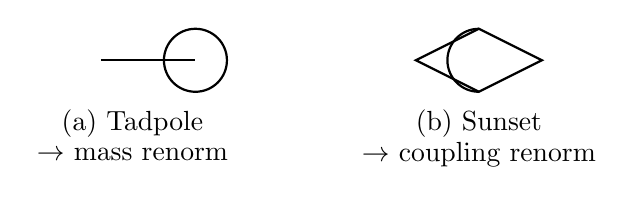
\begin{tikzpicture}[scale=0.8]
% Tadpole for mass
\draw[thick] (-4,0) -- (-2.5,0);
\draw[thick] (-2.5,0) circle (0.5);
\node at (-3.5,-1) {(a) Tadpole};
\node at (-3.5,-1.5) {$\to$ mass renorm};

% Sunset for coupling
\draw[thick] (1,0) -- (2,0.5) -- (3,0) -- (2,-0.5) -- cycle;
\draw[thick] (2,0.5) arc (90:270:0.5);
\node at (2,-1) {(b) Sunset};
\node at (2,-1.5) {$\to$ coupling renorm};
\end{tikzpicture}
\end{center}

\textbf{Mass correction (tadpole):} The vertex $\frac{u_0}{4!}(\phi^a\phi^a)^2$ contains the term $\frac{u_0}{2}(\phi^a\phi^a)\delta^{bc}\phi^b\phi^c$. Contracting two $\phi$ fields in a loop:
\begin{equation}
\delta r = \frac{u_0}{2} \cdot N \cdot \int \frac{d^d k}{(2\pi)^d} \frac{1}{k^2 + r} = \frac{(N+2)u_0}{6} \cdot I_1
\end{equation}
where $I_1 = \int d^dk/(k^2+r)$ has a pole $\sim 1/\varepsilon$ in $d = 4 - \varepsilon$, and the factor $(N+2)$ arises from the O(N) index contractions.

\textbf{Coupling correction (sunset):} The four-point vertex correction involves two internal propagators. After O(N) index algebra:
\begin{equation}
\delta u = -\frac{(N+8)u_0^2}{36} \cdot I_2
\end{equation}
where $I_2$ is the sunset integral, also with a $1/\varepsilon$ pole.

\textbf{Renormalization and beta function:} In the $\overline{\text{MS}}$ scheme, the counterterms cancel the poles. The renormalized couplings satisfy:
\begin{equation}
r_0 = \mu^2 Z_r r, \qquad u_0 = \mu^\varepsilon Z_u u
\end{equation}
with $Z_r = 1 - \frac{(N+2)u}{6(4\pi)^2\varepsilon} + O(u^2)$ and $Z_u = 1 + \frac{(N+8)u}{6(4\pi)^2\varepsilon} + O(u^2)$.

\textbf{The beta function from $\mu\partial_\mu u_0 = 0$:}
\begin{equation}
\beta_u = \mu \frac{\partial u}{\partial \mu} = -\varepsilon u + u \cdot \mu\frac{\partial}{\partial\mu}\ln Z_u = -\varepsilon u + \frac{(N+8)u^2}{6(4\pi)^2}
\end{equation}

\textbf{Physical interpretation:} The $(N+2)$ factor in $\beta_r$ counts the number of field components that can run in the tadpole loop. The $(N+8)$ factor in $\beta_u$ arises from the sum over three distinct index structures in the four-point function.
\end{workedbox}

\subsection{The Nontrivial Fixed Point}

Setting $\beta_u = 0$ in equation~\eqref{eq:beta_u} gives the Wilson-Fisher fixed point:
\begin{equation}
u^* = \frac{6(4\pi)^2 \varepsilon}{N+8} + O(\varepsilon^2).
\label{eq:wilson_fisher}
\end{equation}

\marginnote{The Wilson-Fisher fixed point exists for $\varepsilon > 0$ (i.e., $d < 4$) and governs continuous phase transitions.}

At this fixed point, the stability matrix (equation~\ref{eq:stability_matrix}) has eigenvalues:
\begin{align}
\lambda_r &= 2 - \frac{(N+2)\varepsilon}{N+8} + O(\varepsilon^2), \\
\lambda_u &= \varepsilon + O(\varepsilon^2).
\end{align}

The eigenvalue $\lambda_r > 0$ indicates that $r$ is a relevant perturbation (temperature deviation from criticality). The correlation length exponent is
\begin{equation}
\nu = \frac{1}{\lambda_r} = \frac{1}{2} + \frac{(N+2)\varepsilon}{4(N+8)} + O(\varepsilon^2).
\label{eq:nu_exponent}
\end{equation}

%-------------------------------------------------------------------------------
\section{Critical Exponents and Universality}
\label{sec:on_critical}
%-------------------------------------------------------------------------------

The critical exponents characterize the singular behavior near the phase transition.

\subsection{Standard Critical Exponents}

Near the critical point at $r = r_c$:
\begin{align}
\xi &\sim |r - r_c|^{-\nu}, &&\text{(correlation length)}\\
\chi &\sim |r - r_c|^{-\gamma}, &&\text{(susceptibility)}\\
\langle \phi \rangle &\sim (-r + r_c)^{\beta}, &&\text{(order parameter)}\\
G(r) &\sim r^{-(d-2+\eta)}, &&\text{(correlation function)}
\end{align}

\marginnote{The critical exponents depend only on $d$ and $N$, not on microscopic details. This is universality.}

The anomalous dimension $\eta$ arises from the field renormalization and is given by
\begin{equation}
\eta = \frac{(N+2)\varepsilon^2}{2(N+8)^2} + O(\varepsilon^3).
\end{equation}

This is precisely the anomalous dimension discussed in Chapter~\ref{ch:rg_equation}, arising from the scale dependence of the field normalization.

\subsection{Scaling Relations}

The critical exponents satisfy scaling relations (Chapter~\ref{ch:fixed_points}):
\begin{align}
\gamma &= \nu(2 - \eta), \\
\alpha &= 2 - d\nu, \\
\beta &= \frac{\nu(d - 2 + \eta)}{2}.
\end{align}

These relations are consequences of the RG structure and hold for any fixed point, not just Wilson-Fisher.

%-------------------------------------------------------------------------------
\section{Large-N Limit and the Metric}
\label{sec:large_n}
%-------------------------------------------------------------------------------

The large-N limit provides a solvable example where the geometry of theory space can be computed exactly.

\subsection{Large-N Saddle Point}

In the limit $N \to \infty$ with $u N$ held fixed, the path integral is dominated by a saddle point. Introducing an auxiliary field $\sigma = \phi^a \phi^a$, the effective action becomes
\begin{equation}
S_{\text{eff}}[\sigma] = \frac{N}{2}\left[ \mathrm{Tr}\ln(-\nabla^2 + r + \sigma) - \int d^d x \frac{\sigma^2}{4u} \right].
\end{equation}

The saddle point equation $\delta S_{\text{eff}}/\delta \sigma = 0$ determines the gap equation for the effective mass.

\subsection{Fisher Information Metric}

Following Chapter~\ref{ch:geometry}, we can compute the metric on the space of couplings from the two-point function:
\begin{equation}
G_{ij} = \frac{1}{N}\langle \mathcal{O}_i \mathcal{O}_j \rangle
\end{equation}
where $\mathcal{O}_i$ are operators conjugate to the couplings.

\marginnote{The Fisher information metric coincides with the Zamolodchikov metric in suitable limits.}

In the large-N limit, this metric can be computed explicitly from Gaussian fluctuations around the saddle point. The result takes the form
\begin{equation}
ds^2 = G_{rr}(r, u) dr^2 + 2G_{ru}(r, u) dr\, du + G_{uu}(r, u) du^2
\end{equation}
with specific functions that can be determined from the correlation functions.

%-------------------------------------------------------------------------------
\section{RG Flow as Gradient Flow}
\label{sec:on_gradient}
%-------------------------------------------------------------------------------

For $d = 2$, the O(N) model is a conformal field theory at criticality, and Zamolodchikov's c-theorem applies directly.

\subsection{The c-Function}

Zamolodchikov showed that there exists a function $C(r, u)$ satisfying:
\begin{equation}
\frac{dC}{ds} = -G_{ij}\beta^i \beta^j \leq 0
\end{equation}
where $s = \ln \mu$ is the RG scale.

\marginnote{The c-function monotonically decreases along RG trajectories, proving irreversibility.}

At fixed points, $\beta^i = 0$ and $C$ takes the value of the Virasoro central charge. At the Gaussian fixed point, the central charge is $c = N$, reflecting the $N$ free scalar degrees of freedom. At the Wilson-Fisher fixed point in two dimensions (when it exists), the central charge satisfies $c < N$, reflecting the reduced number of effective degrees of freedom at strong coupling. This demonstrates that the RG flow is always ``downhill'' in the central charge.

\subsection{Connection to Entropy}

The decrease of $c$ can be interpreted as a loss of degrees of freedom under coarse-graining. As we integrate out short-distance fluctuations, the effective theory has fewer active degrees of freedom, just as entropy increases in thermodynamics.

%-------------------------------------------------------------------------------
\section{The Anharmonic Oscillator Revisited}
\label{sec:on_anharmonic}
%-------------------------------------------------------------------------------

The one-dimensional version of the O(N) model with $N=1$ is precisely the anharmonic oscillator introduced in Chapter~\ref{ch:scale}.

\subsection{From Partition Function to RG}

The partition function
\begin{equation}
Z = \int_{-\infty}^{\infty} dx \, e^{-\beta(\frac{1}{2}\omega^2 x^2 + \frac{\lambda}{4}x^4)}
\end{equation}
can be analyzed using the same RG techniques. In zero dimensions (quantum mechanics at finite temperature), there is no momentum integral, so the beta functions arise purely from the measure.

\marginnote{The anharmonic oscillator provides the simplest example of the RG in field theory, with all essential features present.}

\subsection{Strong Coupling Expansion}

For large $\lambda$, the perturbative expansion fails, but the RG allows systematic improvement. The effective coupling at scale $\mu$ satisfies
\begin{equation}
\mu \frac{d\lambda_{\text{eff}}}{d\mu} = \beta_\lambda(\lambda_{\text{eff}})
\end{equation}
which can be integrated to resum the perturbation series.

This is the statistical mechanics analog of the secular term resummation in the ODE version (Chapter~\ref{ch:scale}).

%-------------------------------------------------------------------------------
\section{Connection to the Geometric Framework}
\label{sec:on_geometry}
%-------------------------------------------------------------------------------

We now summarize how the O(N) model illustrates all aspects of the geometric framework.

\subsection{Theory Space}

The coupling space $(r, u)$ is a two-dimensional manifold. The RG flow
\begin{align}
\dot{r} &= \beta_r(r, u), \\
\dot{u} &= \beta_u(r, u)
\end{align}
defines a vector field on this manifold.

\subsection{Fixed Points and Scaling}

The Gaussian and Wilson-Fisher fixed points organize the flow, serving as the endpoints of RG trajectories. The stability matrix at each fixed point determines the local flow structure completely. Its eigenvalues distinguish relevant directions (unstable under the flow) from irrelevant directions (stable under the flow). The critical exponents follow directly from these eigenvalues through the relation $\Delta_a = d - \lambda_a$. The number of relevant perturbations determines the universality class: systems requiring the same number of tuned parameters to reach the fixed point belong to the same class.

\subsection{The Metric}

The Zamolodchikov metric provides a natural Riemannian structure on theory space. The RG flow is a gradient flow with respect to this metric, with the c-function as the potential.

\subsection{Connections}

Scheme changes correspond to coordinate transformations on theory space. The connection (Chapter~\ref{ch:connections}) ensures that physical quantities are scheme-independent.

\subsection{Renormalons and the Mass Gap}

The perturbative $\varepsilon$-expansion for the O(N) model, like all asymptotic series in field theory, exhibits renormalon singularities in its Borel transform. The singularity positions follow from the one-loop beta function coefficient:
\begin{equation}
\zeta_k = \frac{k}{\beta_1} = \frac{6k(4\pi)^2}{N+8}, \qquad k = 1, 2, 3, \ldots
\end{equation}

\marginnote{The renormalon structure of the O(N) model mirrors the general framework of Chapter~\ref{ch:rg_equation}---the positions follow from the RGE, not from summing diagrams.}

These renormalons have physical significance. The dynamically generated mass gap $m_{\text{gap}}$ in the O(N) model (relevant for $N > 2$ in two dimensions) is a non-perturbative effect invisible to any finite order of perturbation theory. It appears in the transseries as:
\begin{equation}
m_{\text{gap}} \sim \Lambda \, e^{-1/(|\beta_1| g_*)}
\end{equation}
where $\Lambda$ is the UV cutoff and $g_*$ is the coupling at the Wilson-Fisher fixed point.

The cancellation of ambiguities between the perturbative series and the mass gap sector illustrates the general principle of Chapter~\ref{ch:rg_equation}: the imaginary parts from Borel resummation must cancel against contributions from non-perturbative sectors for physical observables to be real.

\subsection{Connection to the Three Canonical Examples}

The O(N) model connects intimately to all three canonical examples:

\marginnote{The O(N) model is the ``grown-up'' version of the Part I examples: the oscillator partition function in one dimension, the full $\phi^4$ theory in higher dimensions.}

\textbf{Anharmonic oscillator parallel.} The $d = 1$, $N = 1$ limit of the O(N) model is precisely the partition function of the anharmonic oscillator. The running coupling $u(\Lambda)$ is the field-theoretic generalization of the oscillator's running frequency.

\textbf{$\phi^4$ theory parallel.} The O(N) model \emph{is} $\phi^4$ theory with $N$-component fields. It directly implements all concepts from the $\phi^4$ example: the Gaussian fixed point, the Wilson-Fisher fixed point at $u^* = O(\epsilon)$, and the perturbative beta functions~\eqref{eq:beta_r}--\eqref{eq:beta_u}.

\textbf{PME parallel.} Critical exponents like $\nu = 1/2 + O(\epsilon)$ and $\eta = O(\epsilon^2)$ are anomalous dimensions---they differ from their mean-field values due to fluctuations. The $\epsilon$-expansion gives predictions that must be resummed to apply at physical dimension $d = 3$ ($\epsilon = 1$), exactly as in second-kind self-similarity.

%-------------------------------------------------------------------------------
\section{Summary}
\label{sec:on_summary}
%-------------------------------------------------------------------------------

The O(N) model demonstrates the six-step RG recipe in its natural habitat: statistical field theory near continuous phase transitions. The scale hierarchy (Step 1) extends from the microscopic cutoff $\Lambda$ to the diverging correlation length $\xi$. Perturbative analysis with Borel structure (Step 2) reveals renormalon singularities from RG running. Theory space (Step 3) has coordinates $(r, u)$ with the RG flow defining a vector field, extended to include transseries parameters. The beta functions (Step 4) are computed via the $\epsilon$-expansion, yielding equations~\eqref{eq:beta_r} and~\eqref{eq:beta_u}. Fixed-point analysis (Step 5) reveals the Wilson-Fisher fixed point~\eqref{eq:wilson_fisher} with universal critical exponents. Physical predictions for exponents at $\epsilon = 1$ require Borel resummation (Step 6).

The chapter has invoked every element of the geometric framework from Part I. Canonical scaling dimensions follow from the dilation group analysis of Chapter~\ref{ch:flows}. Beta functions emerge from scale covariance as developed in Chapter~\ref{ch:rg_equation}. Fixed points and stability analysis apply the machinery of Chapter~\ref{ch:fixed_points}. The Zamolodchikov metric and gradient flow structure connect to the geometry of Chapter~\ref{ch:geometry}. The c-theorem establishes irreversibility of the flow.

The one-dimensional limit of the O(N) model with $N=1$ is precisely the anharmonic oscillator partition function that introduced the RG in Chapter~\ref{ch:scale}. This connection closes the pedagogical loop: the abstract framework produces concrete, testable predictions for critical phenomena that agree with experiment to high precision. The correlation length exponent $\nu$ in three dimensions, for example, has been measured in superfluid helium and agrees with the theoretical prediction to several decimal places.

